
\section{Введение и краткая теория}
При дифракции на предмете с периодической структурой наблюдается явление саморепродукции: на некотором расстоянии от предмета вдоль направления распространения волны появляется изображение, которое потом периодически повторяется.  \par
Представим волну за периодическим объектом в виде суммы плоских волн разных направлений. Отдельные слагаемые плоские волны называют пространственными гармониками. Вдоль пути распространения волнового фронта на некотором расстоянии $z_0$ от предмета существует плоскость, где разность фазовых набегов любых пространственных гармоник (плоских волн идущих под углом $\theta$т к оси распространения), входящих в состав суперпозиции, кратна $2T$ В этой плоскости фазовые соотношения между всеми плоскими волнами, входящими в состав суперпозиции, такие же, что и в предметной плоскости. Поэтому в результате интерференции этих волн возникает изображение, тождественное исходному периодическому объекту. Все сказанное справедливо для любого расстояния $z_n$, кратного $z_0$. Для решетки с периодом $d$.
\begin{equation}
    z_n = \frac{2d^2}{\lambda}n
\end{equation}

Суть эксперимента по саморепродукции состоит в том, что дифрагированная на периодическом транспаранте (решетка, сетка) плоская монохроматическая волна лазера (лазерный пучок) воспроизводит изображение транспаранта без каких-либо оптических элементов.

\begin{figure}[h!]
    \centering
    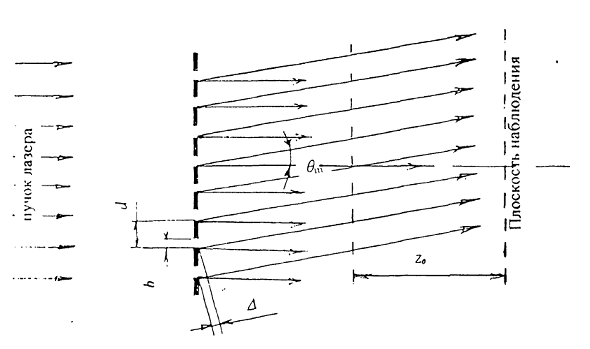
\includegraphics[width=15cm]{pics/fig1.png}
    \caption{Дифракция лучей на сетке и возникновение саморепродуцированного изображения}
    \label{fig:vac}
\end{figure}
